% Kopfzeile beim Kapitelanfang:
\fancypagestyle{plain}{
%Kopfzeile links bzw. innen
\fancyhead[L]{\Large Vorlesung 21 (06.01.2013)}
%Kopfzeile rechts bzw. außen
\fancyhead[R]{}}
%Kopfzeile links bzw. innen
\fancyhead[L]{\Large Vorlesung 21 (06.01.2014)}
%Kopfzeile rechts bzw. außen
\fancyhead[R]{}
% **************************************************
\section{Satz: Ableitung der Umkehrfunktion}\label{11.8}
Sei $f: D \to \R$ stetig und streng monoton, und differenzierbar in $x_0 \in D$ mit $f'(x_0) \neq 0 \Ra$\\
$f^{-1}$ differenzierbar in $y_0 = f(x_0)$ mit \fbox{$(f^{-1})'(y_0)=\frac{1}{f'(x_0)} = \frac{1}{f'(f^{-1}(y_0))}$}\nl
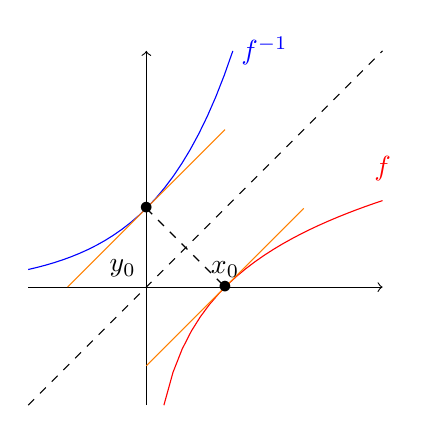
\begin{tikzpicture}
\draw[->] (-1.5,0)--(3,0);
\draw[->] (0,-1.5)--(0,3);
\draw[color=blue,domain=-1.5:1.0986] plot (\x, {exp(\x)}); % f^-1
\draw[color=red,domain=0.22313:3] plot (\x, {ln(\x)}); %f
\draw[dashed] (-1.5,-1.5)--(3,3);
\draw[color=blue] (1.5,3) node {$f^{-1}$};
\draw[color=red] (3,1.5) node {$f$};
\draw[color=orange,domain=-1:1] plot (\x, {\x+1});
\draw[color=orange,domain=0:2] plot (\x, {\x-1});
\draw (0,1) node {$\bullet$};
\draw (1,0) node {$\bullet$};
\draw[dashed] (0,1)--(1,0);
\draw[dashed] (0,1)--(0,0);
\draw (-0.3,0) node[above] {$y_0$};
\draw (1,0) node[above] {$x_0$};
\end{tikzpicture}

\subsection*{Beweis}
Satz \ref{10.3} + Lemma \ref{10.2} $\Ra f: D \to f(D)$ bijektiv, und $f^{-1}$ stetig.\\
Betrachte $y_0, y \in f(D), y \neq y_0, y \to y_0 \Ra x=f^{-1}(y) \to f^{-1}(y_0)=x_0$\\
$\lim_{y \to y_0} \frac{f^{-1}(y) - f^{-1}(y_0)}{y-y_0} = \lim_{x \to x_0} \frac{x-x_0}{f(x)-f(x_0)} = \frac{1}{f'(x_0)}$ \qed

\subsection*{Beispiel}
$\ln y$ ist Umkehrfunktion von $f(x)=e^x, x \in \R$\\
$\Ra \ln'(y) = \frac{1}{\exp'(\ln y)} = \frac{1}{\exp(\ln y)} = \frac{1}{y}$ (wie gehabt)

\phantomsection
\addcontentsline{toc}{section}{Einseitige Ableitungen}
\section*{Einseitige Ableitungen}
Sei $f: D \to \R, x_0 \in D$\\
Existiert nur $\lim_{x \uparrow x_0} \frac{f(x)-f(x_0)}{x-x_0} =: f'_{\text{-}}(x_0)$\\
bzw. $\lim_{x \downarrow x_0} \frac{f(x)-f(x_0)}{x-x_0} =: f'_{\text{+}}(x_0)$,\\
so heißt dieser Grenzwert die linksseitige bzw. rechtsseitige Ableitung von $f$ in $x_0$.

\subsection*{Beispiel}
$f(x)=|x|$ ist nicht differenzierbar in $0$.\nl
$f'_{\text{+}}(0) = \lim_{x \downarrow x_0} \frac{|x|}{x} = 1$\\
$f'_{\text{-}}(0) = \lim_{x \uparrow x_0} \frac{|x|}{x} = -1$\nl
\begin{tikzpicture}
\draw[->] (-2,0)--(2,0);
\draw[->] (0,-0.5)--(0,2);
\draw[color=blue,domain=-2:2] plot (\x, {abs(\x)});
\draw[color=blue] (2,1.5) node {$|x|$};
\end{tikzpicture}

\newpage

\phantomsection
\addcontentsline{toc}{section}{Höhere Ableitungen}
\section*{Höhere Ableitungen}
Betrachte $f: D \to \R, x_0 \in D$, $f$ sei differenzierbar auf einem Intervall $(x_0-\eps, x_0+\eps)$ um $x_0$.\\
Ist $f'$ differenzierbar in $x_0$, so heißt $f$ 2-mal differenzierbar in $x_0$.

\subsection*{Bezeichnung}
$f''(x_0) := \frac{d^2}{dx^2} f(x_0) := (f')'(x_0)$\nl
Für $n \ge 2$: $n$-te Ableitung von $f$ in $x_0$:\\
$f^{(0)}(x_0) := f(x_0)$\\
$f^{(n)}(x_0) := (f^{n-1})'(x_0)$ sofern existent\nl
$f$ heißt dann $n$-mal differenzierbar in $x_0$.

\subsection*{Bezeichnung}
$f$ $n$-mal stetig differenzierbar auf $D :\Lra$\\
$f'=f^{(1)}, f''=f^{(2)}, \ldots, f^{(n)}: D \to \R$ existieren und sind stetig auf $D$.\nl
$C^n(D) := \{f: D \to \R: f \ n\text{-mal stetig differenzierbar}\}$

\section*{Extrema und Mittelwertsatz}
\section{Definition: Extrema}\label{11.9}
Sei $f: D \to \R$ eine Funktion. $f$ hat in $x_0 \in D$ ein
\items{
\item \underline{globales Maximum} $:\Lra f(x) \le f(x_0) \forall x \in D$
\item \underline{lokales Maximum} $:\Lra \exists \eps > 0: f(x) \le f(x_0) \forall x \in D$ mit $|x-x_0| < \eps$
}
Dieses heißt \underline{isoliert}, falls zusätzlich $f(x) < f(x_0) \forall x \in D$ mit $|x-x_0| < \eps, x \neq x_0$.\\
Analog: globales/lokales Minimum.\

\newpage

\section{Notwendiges Kriterium für lokale Extrema}\label{11.10}
Sei $f: (a,b) \to \R$ differenzierbar in $x_0 \in (a,b)$.\\
$f$ habe in $x_0$ lokales Extremum $\Ra f'(x_0) = 0$

\subsection*{Beweis}
$f$ habe in $x_0$ lokales Maximum.\\
$\eps > 0$ klein genug $\Ra \frac{f(x)-f(x_0)}{x-x_0} \left\{\begin{array}{l l} \le 0 & \text{für } x \in (x_0, x_0 + \eps) \\ \ge 0 & \text{für } x \in (x_0-\eps,x_0) \end{array}\right.$
$\Ra f'(x_0) = 0$ \qed\nl
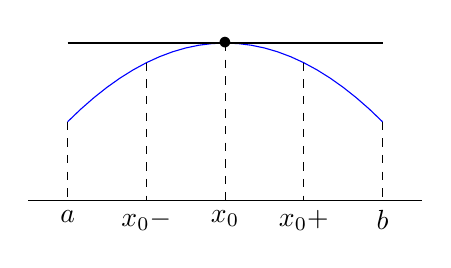
\begin{tikzpicture}
\draw (-2.5,0)--(2.5,0);
\draw[color=blue,domain=-2:2] plot (\x, {-0.25*(abs(\x^2))+2});
\draw[dashed] (-2,1)--(-2,0) node[below] {$a$};
\draw[dashed] (2,1)--(2,0) node[below] {$b$};
\draw[dashed] (0,2)--(0,0) node[below] {$x_0$};
\draw (-2,2)--(2,2);
\draw (0,2) node {$\bullet$};
\draw[dashed] (1,1.75)--(1,0) node[below] {$x_0+\eps$};
\draw[dashed] (-1,1.75)--(-1,0) node[below] {$x_0-\eps$};
\end{tikzpicture}

\subsection*{Beachte}
$f: (a,b) \to \R$ habe in $x_0$ ein lokales Extremum, und $f$ ist differenzierbar in $x_0 \Ra f'(x_0) = 0$\\
Dieses Kriterium ist notwendig, aber nicht hinreichend!

\subsection*{Beispiel}
$f(x)=x^3, f'(0)=0$, aber kein Extremum in $0$\nl
% TODO: Graph von x^3 mit Tangente in 0
\begin{tikzpicture}
\draw[->] (-2,0)--(2,0);
\draw[->] (0,-2)--(0,2);
\draw[color=blue,domain=-1.259921:1.259921] plot (\x, {(\x)^3});
\end{tikzpicture}

\section{Vorgehen bei der Suche nach Extrema}\label{11.11}
Sei $f: [a,b] \to \R$ stetig.\\
Satz von Maximum und Minimum $\Ra f$ nimmt auf $[a,b]$ globales Maximum und globales Minimum an.

\subsection*{Kandidaten}
\ena{
\item Punkte $x \in (a,b)$, wo $f$ differenzierbar mit $f'(x)=0$
\item Randpunkte $a,b$
\item Punkte, in denen $f$ nicht differenzierbar ist
}
Globale/Lokale Extrema durch Vergleich der Funktionswerte\nl
Falls $f: I \to \R$, $I$ unbeschränktes Intervall: Untersuche auch $\lim_{x \to \pm \infty} f(x)$

\newpage

\section{Mittelwertsatz der Differentialrechnung}\label{11.12}
$f: [a,b] \to \R$ sei stetig auf $[a,b]$ und differenzierbar auf $(a,b)$\\
$\Ra \exists \xi \in (a,b):$ \fbox{$f'(\xi) = \frac{f(b)-f(a)}{b-a}$} (Steigung der Sekanten)\nl
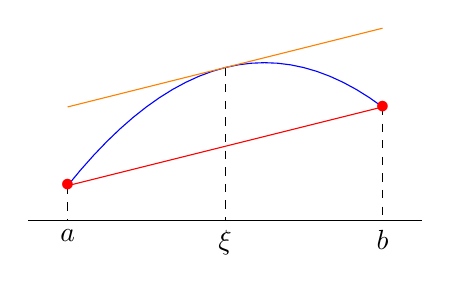
\begin{tikzpicture}
\draw (-2.5,0)--(2.5,0);
\draw[color=blue,domain=-2:2] plot (\x, {-0.25*(abs((\x-0.5)^2))+2});
\draw[dashed] (-2,0.4375)--(-2,0) node[below] {$a$};
\draw[dashed] (2,1.4375)--(2,0) node[below] {$b$};
\draw[color=red] (-2,0.4375)--(2,1.4375);
\draw[color=red] (-2,0.4375) node {$\bullet$};
\draw[color=red] (2,1.4375) node {$\bullet$};
\draw[dashed] (0,1.9375)--(0,0) node[below] {$\xi$};
\draw[color=orange,domain=-2:2] plot (\x, {1/4*\x+1.9375});
\end{tikzpicture}

\phantomsection
\addcontentsline{toc}{subsection}{Satz von Rolle}
\subsection*{Spezialfall: Satz von Rolle}
Ist zusätzlich $f(a)=f(b) \Ra \exists \xi \in (a,b): f'(\xi) = 0$.

\subsection*{Beweis}
\enR{
\item Für Rolle: $f$ stetig auf $[a,b] \Ra f$ nimmt auf $[a,b]$ ein globales Maximum und Minimum an.\\
Falls beide am Rand $\underset{f(a)-f(b)}{\Ra} f=$ konst. $\Ra f'=0$ auf $(a,b)$ (fertig).\\
Andernfalls nimmt $f$ ein Extremum in einem $\xi \in (a,b)$ an $\Ra f'(\xi)=0$
\item Reduktion des Mittelwertsatzes auf Rolle:\\
Betrachte: $g(x) := f(x)-\frac{f(b)-f(a)}{b-a}(x-a)$\\
$\Ra g(a) = f(a) = g(b) \Ra g$ erfüllt Voraussetzung von Rolle\\
$\Ra \exists \xi \in (a,b): 0 = g'(\xi) = f'(\xi) - \frac{f(b)-f(a)}{b-a}$
} \qed

\newpage

\section{Monotonieverhalten differenzierbarer Funktionen}\label{11.13}
Sei $f: (a,b) \to \R$ differenzierbar, $-\infty \le a < b \le +\infty$
\en{
\item $f' > 0$ auf $(a,b) \Ra f$ s.m.w. auf $(a,b)$
\item $f' < 0$ auf $(a,b) \Ra f$ s.m.f. auf $(a,b)$
\item $f' \ge 0 \Lra f$ monoton wachsend auf $(a,b)$
\item $f' \le 0 \Lra f$ monoton fallend auf $(a,b)$
\item $f' \equiv 0 \Lra f$ monoton wachsend und monoton fallend $\Lra f$ konstant auf $(a,b)$
}
Falls $f$ stetig auf ganz $[a,b]$, so gelten die Aussagen über Monotonie und Konstanz auf dem abgeschlossenen Intervall $[a,b]$.

\subsection*{Beweis}
Sei $a < x < y < b$ (bzw. $a \le x < y \le b$ falls $f$ stetig auf $[a,b]$)\\
MWS $\Ra \frac{f(y)-f(x)}{y-x} = f'(\xi)$ mit geeignetem $\xi \in (x,y)$
\en{
\item $f'(\xi) > 0 \Ra f(y) > f(x) \Ra f$ s.m.w.
\item und "`$\Ra$"' in (3),(4) analog
}
Zu "`$\La$"' in (3): Sei $x \in (a,b) \Ra f'(x) = \lim_{y \downarrow x} \frac{f(y)-f(x)}{y-x} \ge 0$\\
(4) analog, (5) aus (3)+(4) \qed

\subsection*{Beachte}
In (1),(2) gilt nicht "`$\La$"'.
\underline{Beispiel}: $f(x)=x^3$, s.m.w. auf $\R^3$, $f'(0)=0$

\subsection*{Anwendung von (5)}
Betrachte $f(x)=e^{ax}, f'(x)=a \cdot e^{ax} = a \cdot f(x)$\\
Das heißt, $f(x)=e^{ax}$ genügt der Differentialgleichung $f'=af$ auf $\R$

\section{Korollar}\label{11.14}
$f: \R \to \R$ sei differenzierbar und erfülle $f'=af$ auf $\R$ mit einer Konstanten $a \in \R \Ra f(x)=c \cdot e^{ax}$ mit $c = f(0)$

\subsection*{Beweis}
Trick: $g(x) := e^{-ax} f(x) \underset{\text{Produktr.}}{\Ra} g'(x) = -ae^{-ax} f(x) + e^{-ax} \overbrace{f'(x)}^{af(x)} = 0$\\
$\underset{(5)}{\Ra} g =$ konstant $= g(0) = f(0) = c$ \qed